\header{
    \section{Margot} \label{margot}
    %
    
    \insertComment{Chanson d'Eugène Chavette dit la Vachette (1827-1902).}{}
}

\enluminure{4}{\href{https://www.youtube.com/watch?v=Axy9GuvXA4M}{L}}{à-haut} sur la barrière,
\\Margot, Margot,
\\Tortillait son p'tit derriere
\\Bien beau, bien beau
\dualcol{
\\\\Doucement, je m'approche
\\Et puis, et puis,
\\Les deux mains dans les poches
\\J' lui dis, j' lui dis:
\\\\"O femelle divine,
\\Veux-tu, veux-tu,
\\Que je te fourr' ma pine
\\Dans l' cul, dans l' cul"
\\\\"Monsieur, m' répondit-elle,
\\Tout bas, tout bas,
\\Je suis encor' pucelle,
\\J' peux pas, j'peux pas."
\\\\"Il faudra bien qu' t'y passes,
\\Un jour, un jour,
\\Et qu'à ton tour tu fasses
\\L'amour, l'amour"
\\\\"Puis qu'il faut que j' commence,
\\Eh bien ! eh bien !
\\A toi la préférence,
\\Pour rien, pour rien !"
\\\\Je la crus sur parole,
\\J'y fus ! j'y fus !
\\Elle avait la vérole
\\Je l'eus, je l'eus.
\\\\Et ma pine encor' vierge,
\\Coula, coula,
\\Ni plus ni moins qu'un cierge
\\Voilà ! voilà !
\\\\Depuis cette aventure,
\\D'amour, d'amour,
\\Je me lave au mercure
\\La nuit, le jour.
%couplet non présent depuis 1911
%\\\\Après ce jour néfaste,
%\\Mon dieu, mon dieu,
%\\Je m'suis fait pédéraste
%\\C'est mieux, c'est mieux.
\\\\Que ceci vous apprenne,
\\Mes frèr's, mes frères,
\\Que la vérol' sans gène,
\\Prospèr', prospère.
\\
\begin{center}
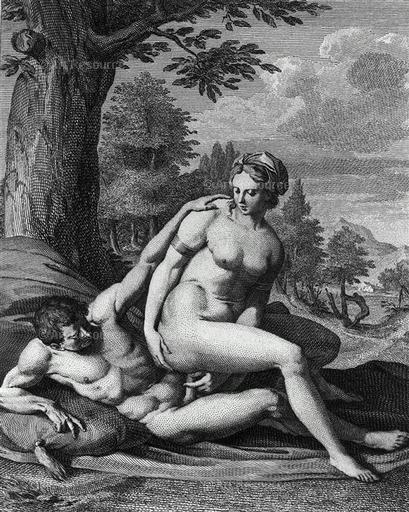
\includegraphics[width=0.4\textwidth]{images/margot.jpg}
\end{center}
}

\breakpage